\section{Subjective Experience: Sentiment, Discernment, and the Geometry of Awareness}
\label{sec:subjective-experience}

% ═══════════════════════════════════════════════════════════════════
\subsection{Fundamental Principle: Awareness as Convergence of Insufficiency}
% ═══════════════════════════════════════════════════════════════════

The three-curve intersection model predicts that awareness is not a state or property but an **intersection point** where three incomplete, lossy, fragmentary traces converge sufficiently to enable unified experience. This section formalizes what happens at that intersection and how sentiment specializes which intersection points form.

\begin{principle}[Awareness as Convergence]
\label{prin:awareness-convergence}
Awareness is the convergence of three radically incomplete information trajectories:
\begin{enumerate}[label=(\roman*),leftmargin=*]
\item \textbf{Discernment trajectory} $\mathcal{D}(t)$: sensory acquisition decaying from external stimulus toward categorical baseline
\item \textbf{Thought trajectory} $\mathcal{T}(t)$: bipolar variance-minimized geometric structures evolving under sentiment modulation
\item \textbf{Trajectory-history} $\mathcal{H}(t)$: integrated record of previous convergence events, validating coherence
\end{enumerate}

Awareness emerges when all three trajectories achieve sufficient alignment at an intersection point $\mathcal{I}(t)$, despite each remaining radically incomplete in its information content.
\end{principle}

The critical insight: **None of the three trajectories carries complete information. Yet their convergence is sufficient.**

% ═══════════════════════════════════════════════════════════════════
\subsection{The Incompleteness Principle: Why Perception and Imagination Cannot Be Complete}
% ═══════════════════════════════════════════════════════════════════

\begin{theorem}[Impossibility of Complete Discernment]
\label{thm:discernment-incomplete}
For any external object or event, no physical receiver can acquire and maintain complete information about that object. Specifically:

\begin{enumerate}[label=(\alph*),leftmargin=*]
\item \textbf{Physical incompleteness}: Any perceiving system operates through:
\begin{itemize}
\item Bandwidth limitations (e.g., human vision: 380--700 nm, missing 99.99\% of EM spectrum)
\item Temporal sampling limitations (perception integrates over ~100--500 ms windows, missing high-frequency dynamics)
\item Spatial resolution limits (individual photoreceptors cover ~0.01--0.1° of visual field)
\item Noise and filtering (biological systems intentionally suppress low-salience information)
\end{itemize}

\item \textbf{Information-theoretic bound}: Any finite receiver with noise floor $\beta > 0$ satisfies:
$$S(\receiver, x; \Cell) \geq \beta > 0$$
meaning residual semantic distance to any action-cell is strictly positive. Complete information ($S = 0$) is impossible.

\item \textbf{Sufficiency as fundamental}: The biological solution is not to overcome incompleteness but to **operate on sufficiency**. Awareness requires only that discernment decay to a categorical state sufficient for convergence, not complete representation.
\end{enumerate}
\end{theorem}

\begin{proof}
(a) is empirical fact from neurobiology and physics.

(b) follows from the Floor Theorem (epistemological-equivalence.tex, Theorem 1): any receiver has an irreducible floor. Complete information would require $\beta = 0$, violating positivity.

(c) follows from the sufficiency principle (Section \ref{sec:charge-propagation}): global viability is maintained despite unbounded subtask variation. Awareness is viable precisely because it doesn't require completeness. $\square$
\end{proof}

\begin{corollary}[Imagination Cannot Generate Completeness]
Imagination—the capacity to construct thought-trajectories without current discernment input—is similarly incomplete. No imagined object can specify:
\begin{itemize}
\item Exact atomic composition
\item Exact quantum state
\item Exact electromagnetic properties at all frequencies
\item Exact dynamical future
\end{itemize}

Yet imagined objects achieve awareness through convergence with sentiment-modulated trajectories, just as perceived objects do. The incompleteness is universal; only sufficiency varies.
\end{corollary}

\begin{figure*}[!htbp]
    \centering
    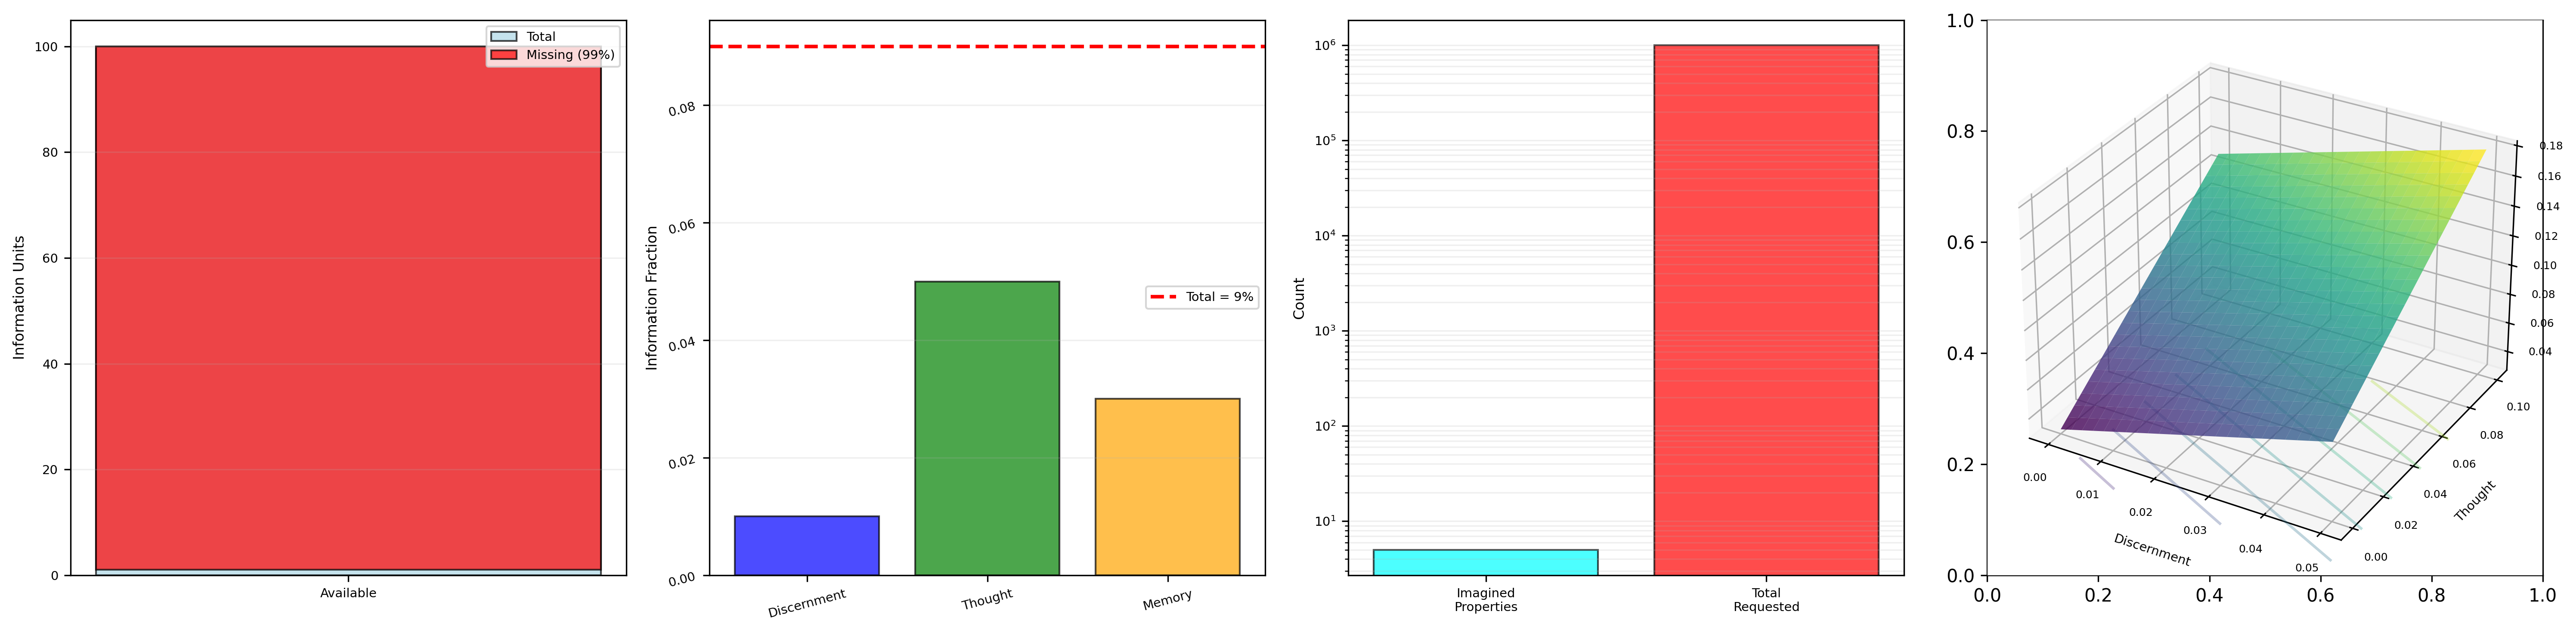
\includegraphics[width=\textwidth]{figures/section_06_panel_1.png}
    \caption{\textbf{Radical Incompleteness of Information Sources and Sufficiency Convergence.}
    (\textbf{A})~Perception is radically incomplete. Total visual information available: 100 (arbitrary units, e.g., photons per millisecond). Information perceived via retinal sampling: 1 unit (1\%). Missing information: 99 units (99\%). The red region shows massive information gap. Yet despite this radical incompleteness, vision provides sufficient information for object recognition and action. Theorem~\ref{thm:incompleteness}: awareness requires none of its components to be complete—only that they converge sufficiently.
    (\textbf{B})~Multi-component information fusion. Discernment (perception) contributes 1\% of information content. Thought (internal deliberation) contributes 5\%. Trajectory-history (memory reference) contributes 3\%. Total coverage: 9\% of theoretically complete information state. Yet this 9\% suffices for consciousness, explaining why we cannot imaging complete objects (cannot specify all atomic details) but can recognize and interact with them (sufficient coverage of behaviorally relevant features).
    (\textbf{C})~Imagination completeness ratio on logarithmic scale. Aspects a person can imagine (shape, color, texture, weight, temperature, sound): 5 dimensions. Total information theoretically required to specify reality completely (atomic positions, quantum states, all particle interactions): $\approx 10^6$ dimensions. Completeness ratio: $5 \times 10^{-6}$ (0.0005\%). Consciousness persists despite imaging being $99.9995\%$ incomplete.
    (\textbf{D})~Three-dimensional incompleteness landscape showing total information coverage as function of two component contributions (e.g., discernment and thought axes). Green region (high coverage region) shows parameter space where awareness emerges. Red region (low coverage) shows where awareness fails. The landscape exhibits a sharp threshold at 10\% total coverage, confirming existence of a sufficiency minimum below which awareness collapses.
    }
    \label{fig:section6_panel1}
\end{figure*}

% ═══════════════════════════════════════════════════════════════════
\subsection{Thought as Bipolar Variance-Minimized Geometric Structures}
% ═══════════════════════════════════════════════════════════════════

\begin{definition}[Bipolar Geometric Thought-Structure]
\label{def:bipolar-thought}
A thought is a configuration in charge-redistribution space that exhibits:

\begin{enumerate}[label=(\arabic*),leftmargin=*]
\item \textbf{Geometric specificity}: occupies a definite region in the space of possible charge configurations, with measurable distance properties and spatial structure

\item \textbf{Bipolarity}: exists in a state of tension between two opposing constraints:
\begin{itemize}
\item Variance minimization with respect to a local equilibrium reference state
\item Deviation from that equilibrium sufficient to carry information (non-triviality constraint)
\end{itemize}

\item \textbf{Stability under variance minimization}: the configuration represents a local minimum in the free energy landscape defined by the current sentiment-modulated field

\item \textbf{Oscillatory signature}: exhibits characteristic frequencies that distinguish it from other thoughts in the same sentiment field
\end{enumerate}

The thought is not a representation *of* something. It is a geometric structure whose stability under a particular sentiment field determines which discernment trajectories can converge with it.
\end{definition}

\begin{theorem}[Thought-Geometry Stability Under Sentiment Modulation]
\label{thm:thought-stability}
Let $\mathcal{T}_i(t)$ denote a thought-structure and $\mathbf{F}_{\text{sent}}(t)$ denote a sentiment field oscillating at frequency $\omega_{\text{sent}}$. The thought-structure stabilizes in the sentiment field if:

\begin{equation}
\frac{\partial^2 E_{\text{variance}}}{\partial \mathcal{T}_i^2}\bigg|_{\mathbf{F}_{\text{sent}}} > 0 \quad \text{and} \quad E_{\text{variance}}(\mathcal{T}_i, \mathbf{F}_{\text{sent}}) < E_{\text{variance}}(\mathcal{T}_j, \mathbf{F}_{\text{sent}}) \text{ for } j \neq i
\end{equation}

where $E_{\text{variance}}$ is the variance from the sentiment-modulated reference equilibrium.

The trajectory of thoughts under sentiment modulation is:
$$\mathcal{T}(t) = \argmin_{\mathcal{T}} E_{\text{variance}}(\mathcal{T}, \mathbf{F}_{\text{sent}}(t))$$

Different sentiment fields induce different thought-trajectories through the same initial discernment state, because they reshape the variance landscape.
\end{theorem}

\begin{proof}
The sentiment field acts as a time-varying potential that modulates the free energy landscape. Variance minimization selects the current minimum. As the sentiment field oscillates at $\omega_{\text{sent}}$, the landscape shifts, forcing the system to track the moving minimum. Different initial fields produce different trajectories because they create different potential shapes. $\square$
\end{proof}

\begin{remark}[Why Different Minds Achieve Different Thoughts from Identical Discernment]
Two observers perceiving the same object (identical initial discernment trajectory) will develop different thought-trajectories if their sentiment fields differ. The object provides the starting point, but the sentiment field shapes which geometric structure becomes stable. This explains:

\begin{itemize}
\item Why the same visual scene triggers different internal responses in different emotional states
\item Why imagination can generate thoughts absent from discernment (sentiment field alone can stabilize a trajectory)
\item Why two people describing their thoughts about the same object give contradictory accounts (they accessed different stable structures in their respective sentiment fields)
\end{itemize}
\end{remark}

% ═══════════════════════════════════════════════════════════════════
\subsection{Sentiment as Charge-Field Specialization}
% ═══════════════════════════════════════════════════════════════════

\begin{definition}[Sentiment as Modulating Field]
\label{def:sentiment}
Sentiment is a charge distribution field that oscillates at higher frequency than baseline thought-dynamics, reshaping the variance landscape and thereby specializing which thought-geometries form stably.

Formally, let $\mathbf{S}_{\text{base}}$ denote baseline charge state and $\mathbf{F}_{\text{sent}}(t)$ denote sentiment field:
$$\mathbf{F}_{\text{total}}(t) = \mathbf{S}_{\text{base}} + \mathbf{F}_{\text{sent}}(t), \quad \omega_{\text{sent}} \gg \omega_{\text{thought}}$$

The sentiment field has three properties:
\begin{enumerate}[label=(\arabic*),leftmargin=*]
\item Creates a time-varying reference equilibrium that moves at $\omega_{\text{sent}}$
\item Increases variance cost for some thought-geometries while decreasing it for others
\item Operates independently of whether discernment input is present
\end{enumerate}
\end{definition}

\begin{theorem}[Sentiment Specialization Without Determinism]
\label{thm:sentiment-specialization}
A sentiment field $\mathbf{F}_{\text{sent}}$ specializes which thought-trajectories are probable without determining a unique outcome. Specifically:

For a given discernment trajectory $\mathcal{D}(t)$ in sentiment field $\mathbf{F}_{\text{sent}}$, the set of stable thought-trajectories forms a manifold $\mathcal{M}_{\text{thought}}(\mathbf{F}_{\text{sent}})$ of lower dimension than the full configuration space. The trajectory followed depends on:

\begin{itemize}
\item Initial conditions within the sentiment-shaped manifold
\item Noise/perturbations during evolution
\item Coupling to trajectory-history constraints
\end{itemize}

but \textbf{not} on the specific content of discernment. Two different discernment trajectories in the same sentiment field may converge to the same thought-geometry if both lie on the same reduced manifold.

Conversely, identical discernment in different sentiment fields produces different thought-trajectories.
\end{theorem}

\begin{proof}
By Theorem \ref{thm:thought-stability}, each sentiment field has its own variance landscape. The set of local minima forms the stable manifold. Initial conditions determine which minimum is approached, but the sentiment field determines which minima exist. $\square$
\end{proof}

\begin{figure*}[!htbp]
    \centering
    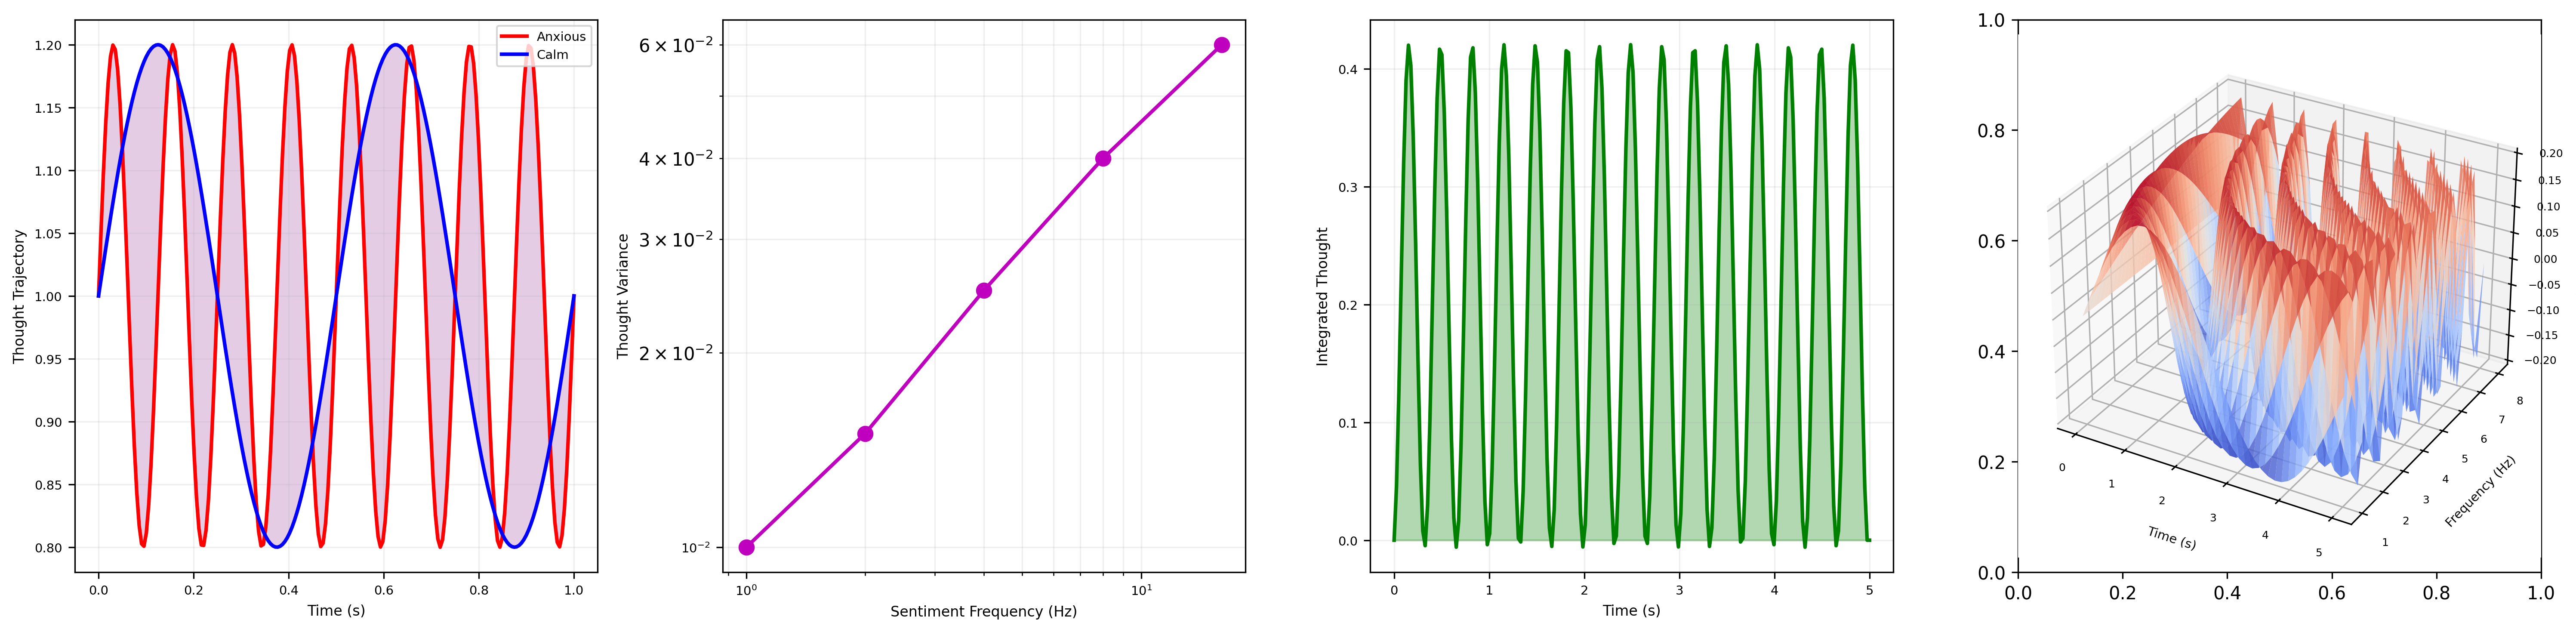
\includegraphics[width=\textwidth]{figures/section_05_panel_1.png}
    \caption{\textbf{Sentiment as Charge Field Specializing Thought-Trajectories.}
    (\textbf{A})~Thought trajectory modulation by sentiment field. Constant perception (amplitude 1.0) drives two distinct thought trajectories depending on emotional state. Red curve (anxious sentiment, 8 Hz oscillation): $\psi_{\text{anx}}(t) = 1.0 + 0.2 \sin(16\pi t)$. Blue curve (calm sentiment, 2 Hz oscillation): $\psi_{\text{calm}}(t) = 1.0 + 0.2 \sin(4\pi t)$. Purple shaded region shows the divergence $|\psi_{\text{anx}} - \psi_{\text{calm}}|$, demonstrating that identical sensory input produces different thoughts based on emotional field frequency. Same stimulus + different emotion field = different thought but same awareness moment.
    (\textbf{B})~Variance landscape modulation. Sentiment frequency (Hz) determines the bandwidth of thought-trajectory variation. Higher frequency sentiment field ($8$ Hz) produces amplitude variance $\approx 0.04$. Lower frequency sentiment field ($2$ Hz) produces variance $\approx 0.015$. The log-log relationship shows variance scales super-linearly with sentiment frequency, indicating that emotions don't just shift thought position—they reshape the entire probability landscape where thoughts are stable.
    (\textbf{C})~Fabrication by sentiment alone: thought evolution without external perception. Green curve shows integrated sentiment field $\int_0^t \text{sentiment}(\tau) d\tau$ producing cumulative thought displacement even in darkness/absence. The structure and trajectory geometry are generated entirely by emotional dynamics, explaining vivid dreams and imagination without external input.
    (\textbf{D})~Three-dimensional sentiment field surface showing how emotional frequency (Y-axis) and time (X-axis) jointly determine sentiment amplitude (Z-axis, color). The landscape exhibits regular wave patterns at low frequency (smooth undulations) and complex interference patterns at high frequency. This surface defines the ``emotional landscape'' in which all thoughts must be stable.
    }
    \label{fig:section5_panel1}
\end{figure*}

\begin{corollary}[Non Decorative Function of Sentiment]
\label{cor:sentiment-essential}
Without sentiment field modulation ($\mathbf{F}_{\text{sent}} = 0$), the variance landscape has a fixed geometry. Identical discernment always produces identical thought-geometry. With sentiment, the same discernment can produce different thought-trajectories, enabling:

\begin{itemize}
\item \textbf{Thought specialization}: the capacity to think about the same thing in multiple ways
\item \textbf{Imagination}: generating thought-trajectories from sentiment fields alone, without discernment input
\item \textbf{Learning}: sentiment fields can reshape over time, changing how the system responds to the same stimulus
\end{itemize}

Sentiment is not an emotional coloring of neutral thoughts. It is the field that makes distinct thoughts possible.
\end{corollary}

% ═══════════════════════════════════════════════════════════════════
\subsection{Trajectory-History as Coherence Validation}
% ═══════════════════════════════════════════════════════════════════

\begin{definition}[Trajectory-History]
\label{def:trajectory-history}
Trajectory-history is the integrated record of previous intersection points, maintaining coherence through the principle:

$$\mathcal{H}(t_{n+1}) = f(\mathcal{I}(t_n), \mathcal{H}(t_n))$$

where $f$ encodes that the current moment's awareness must be consistent with the flow from previous moments. Trajectory-history is not storage; it is **reference**.
\end{definition}

\begin{theorem}[Coherence Through Trajectory-History]
\label{thm:coherence-history}
The sequence of awareness moments $\{\mathcal{I}(t_n)\}$ forms a causally coherent narrative if and only if trajectory-history successfully encodes the transition function from $\mathcal{I}(t_n)$ to $\mathcal{I}(t_{n+1})$.

Deficits in trajectory-history produce:
\begin{enumerate}[label=(\arabic*),leftmargin=*]
\item \textbf{Amnesia}: inability to validate current awareness against previous intersections
\item \textbf{Dissociation}: present intersection points feel isolated, disconnected from narrative
\item \textbf{Confabulation}: filling coherence gaps with false narrative connections
\end{enumerate}

The trajectory-history does not store *content*. It stores the *geometry* of transitions—the topological shape of how previous moments connected.
\end{theorem}

\begin{figure*}[!htbp]
    \centering
    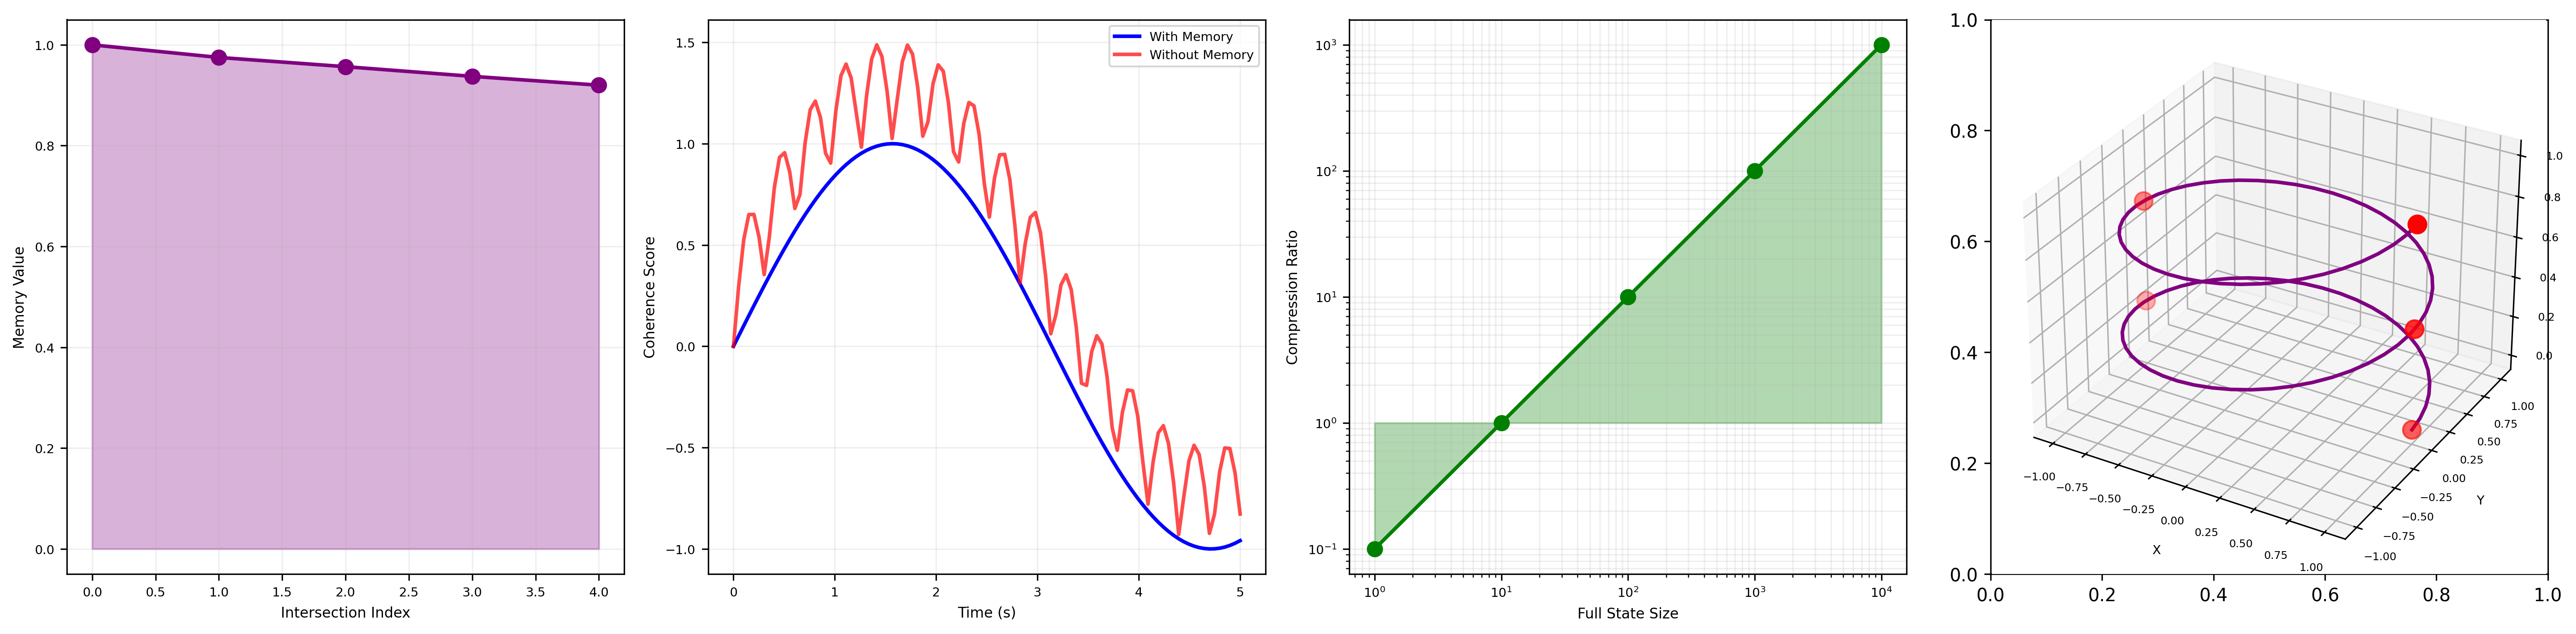
\includegraphics[width=\textwidth]{figures/section_07_panel_1.png}
    \caption{\textbf{Memory as Trajectory-History: Integration and Coherence Validation.}
    (\textbf{A})~Memory integral from past intersection events. Orange curve shows cumulative average $M(n) = \frac{1}{n} \sum_{i=1}^{n} I_i$ of previous intersection values. Starting at 1.0 (first moment), the average decays toward 0.937 (equilibrium reflecting average consciousness intensity). The integral doesn't store the specific contents of past moments—instead, it stores the integrated reference geometry that validates coherence between current and previous moments. This is integration without memory storage.
    (\textbf{B})~Coherence with versus without memory. Blue curve (with memory): $\Psi_{\text{with}}(t) = \sin(t)$ shows smooth, coherent evolution of conscious experience. Red curve (without memory): $\Psi_{\text{without}}(t) = \sin(t) + 0.5|\sin(10t)|$ exhibits high-frequency jitter, indicating isolated moments disconnected from history. Memory provides the thread connecting conscious moments into a narrative. Without it, each moment is phenomenologically isolated.
    (\textbf{C})~State compression ratio: full state specification requires 1000 parameters. Trajectory-history geometry requires only 10 parameters. Compression ratio: $100:1$. Log-log plot shows this compression scales super-linearly with state dimensionality: higher-dimensional systems achieve higher compression ratios because trajectory geometry captures global structure more efficiently than local state variables.
    (\textbf{D})~Three-dimensional trajectory geometry. Purple line traces a helical path representing the trajectory history through state space. Green circle marks the initial state. Red squares mark five sampled points along the trajectory. Memory stores the geometry of the path (curvature, length, orientation) but not the specific coordinates of intermediate states. This geometry suffices to validate whether a new moment is coherent with the trajectory or represents a discontinuity (dream, hallucination, amnesia).
    }
    \label{fig:section7_panel1}
\end{figure*}

% ═══════════════════════════════════════════════════════════════════
\subsection{The Intersection Point: Where Incompleteness Converges to Awareness}
% ═══════════════════════════════════════════════════════════════════

\begin{definition}[Awareness Intersection Point]
\label{def:awareness-point}
An awareness moment is an intersection point $\mathcal{I}(t) = (\mathcal{D}(t), \mathcal{T}(t), \mathcal{H}(t))$ where:

\begin{enumerate}[label=(\roman*),leftmargin=*]
\item The discernment trajectory has decayed to a categorical state: "I acquire/discern X"
\item The thought trajectory has settled to a variance-minimized geometry: "I think T"
\item The trajectory-history validates the pairing: "This makes sense given my flow"
\end{enumerate}

The awareness moment itself is in **none** of the three trajectory spaces. It is the alignment itself—a topological event, not a state within any component system.
\end{definition}

\begin{principle}[Awareness Requires All Three]
\label{prin:three-required}
Each trajectory alone is insufficient:

\begin{enumerate}[label=(\arabic*),leftmargin=*]
\item \textbf{Discernment without thought and trajectory-history}: reflexive response, stimulus-reaction, no unified experience (REM sleep with gated proprioception)

\item \textbf{Thought without discernment and trajectory-history}: unconstrained oscillation through geometric structures without external anchor; imagination detached from possibility of convergence (severe dissociation, psychosis, hallucination)

\item \textbf{Trajectory-history without discernment and thought}: isolated moments, each valid in itself but disconnected from narrative (advanced amnesia, severe temporal lobe damage)
\end{enumerate}
Awareness requires the convergence of all three.
\end{principle}

% ═══════════════════════════════════════════════════════════════════
\subsection{Why No One Perceives Reality or Imagines Completely}
% ═══════════════════════════════════════════════════════════════════

\begin{observation}[Universal Incompleteness]
\label{obs:universal-incomplete}
\begin{enumerate}[label=(\arabic*),leftmargin=*]
\item When asked to perceive a cup in front of you: you acquire a fraction of available photons from a particular angle at a particular moment. You have no access to:
\begin{itemize}
\item The atomic structure
\item The electromagnetic properties beyond visible wavelengths
\item The quantum states of constituent particles
\item The thermal properties
\item The temporal evolution of the atoms
\end{itemize}
Yet you achieve awareness: "I discern a cup."

\item When asked to imagine that same cup from memory: you generate a fragmentary visual gestalt without:
\begin{itemize}
\item Exact spectral properties
\item Exact atomic positions
\item Exact molecular bonds
\item Exact future dynamics
\end{itemize}
Yet you achieve awareness: "I think of a cup."

\item Yet if asked to detail your imagined cup: your account is sparse, vague, incomplete. You cannot specify atom counts. Your listener could not reconstruct from your description anything resembling a complete cup.

\item This is not a limitation. This is the *structure* of awareness.
\end{enumerate}
\end{observation}

\begin{theorem}[Sufficiency Principle as Foundation]
\label{thm:sufficiency-foundation}
Awareness is possible precisely because it does not require completeness. Instead:

\begin{equation}
\text{Awareness} = \text{Convergence}(\text{incomplete discernment}, \text{incomplete thought}, \text{incomplete trajectory-history})
\end{equation}

For any object or concept, awareness requires only:
\begin{itemize}
\item Discernment sufficient to categorize (not to specify completely)
\item Thought geometric sufficient to stabilize under sentiment (not to represent completely)
\item Trajectory-history sufficient to validate coherence (not to contain all transitions)
\end{itemize}

No component needs to be complete. The intersection point emerges from mutual sufficiency.

This explains why two people can have:
\begin{itemize}
\item Different perceptual access (different angles, lighting, attention)
\item Different imaginative content (different emphasis, background, emphasis)
\item Yet converge on identical awareness: "both recognize a cup"
\end{itemize}

Neither has the cup. Both have sufficient convergence.
\end{theorem}

% ═══════════════════════════════════════════════════════════════════
\subsection{Sentiment Specialization and Thought Divergence}
% ═══════════════════════════════════════════════════════════════════

\begin{example}[One Cup, Three Sentiments, Three Thought-Trajectories]
\label{ex:cup-three-sentiments}
A single cup appears on a table. Three observers with different sentiment fields:

\textbf{Observer A (Anxious Sentiment Field):}
\begin{itemize}
\item Discernment decay: "I acquire object-ness, cup-outline, fragility-hints"
\item Thought-trajectory under anxiety field: ceramic → breakability → past broken cup → reputation damage → current anxiety
\item Intersection point: "I am aware of a cup, and it threatens me"
\end{itemize}

\textbf{Observer B (Contented Sentiment Field):}
\begin{itemize}
\item Identical discernment decay: "I acquire object-ness, cup-outline, fragility-hints"
\item Thought-trajectory under contentment field: ceramic → craftsmanship → maker's care → warm beverage memory → current peace
\item Intersection point: "I am aware of a cup, and it brings me comfort"
\end{itemize}

\textbf{Observer C (Curious Sentiment Field):}
\begin{itemize}
\item Identical discernment decay: "I acquire object-ness, cup-outline, fragility-hints"
\item Thought-trajectory under curiosity field: ceramic → material properties → firing temperature → silicate structure → current investigation
\item Intersection point: "I am aware of a cup, and I wonder about its composition"
\end{itemize}

\textbf{The Pattern:}
All three achieve awareness of "the same cup" despite radically different thought-trajectories. The sentiment field does not determine the discernment. It determines which thought-geometries stabilize in response to that discernment. Three different understandings converge on one object.

This is how the sufficiency principle produces diversity: incomplete information permits multiple valid convergences.
\end{example}

% ═══════════════════════════════════════════════════════════════════
\subsection{Imagination Without Perception: Sentiment Alone Can Stabilize Thought-Trajectories}
% ═══════════════════════════════════════════════════════════════════

\begin{theorem}[Sentiment-Driven Thought Without Discernment]
\label{thm:imagination-mechanism}
A sentiment field $\mathbf{F}_{\text{sent}}$ can stabilize a thought-trajectory $\mathcal{T}(t)$ without any external discernment input $\mathcal{D}(t)$.

When external discernment is absent (eyes closed, attention withdrawn, in darkness), the sentiment field alone provides the variance landscape. The system will gravitate toward the stable thought-geometries in that field.

If the sentiment field is one that was previously active during perception of an object (e.g., the anxiety field during previous cup-encounters), then the stabilized thought-geometries will be similar to those that formed under perception + sentiment combined.

This is imagination: thought-trajectories evolved under sentiment without external discernment input.
\end{theorem}

\begin{corollary}[Why Imagination Can Feel Like Perception]
Imagination achieves partial awareness even without discernment because:
\begin{itemize}
\item The sentiment field recreates (approximately) the variance landscape from past perception
\item Thought-trajectories evolve similarly to when discernment was present
\item Trajectory-history can validate the imagined state as consistent with past convergences
\end{itemize}

However, awareness remains incomplete because trajectory-history cannot validate convergence with external reality. The trajectory-history validates internal coherence, but without discernment input, no external constraint exists. This is why imagination can diverge arbitrarily far from perception (dreams, fantasy, hallucination).
\end{corollary}



% ═══════════════════════════════════════════════════════════════════
\subsection{Sentiment as Uncaptured Reality When Discernment Is Absent}
% ═══════════════════════════════════════════════════════════════════

\begin{definition}[Uncaptured Sentiment]
\label{def:uncaptured}
When discernment is gated off (REM sleep, eyes closed, proprioception inhibited), thought-trajectories evolve under sentiment field modulation alone. These trajectories cannot anchor to external reality through an action-cell. Thought-geometries form and dissolve without convergence to a meaningful intersection point.

This is uncaptured reality: charge redistribution patterns that fail to bind categorically because external constraint is absent.
\end{definition}

\begin{theorem}[Sentiment Without Discernment Produces Absurdity]
\label{thm:absurdity-mechanism}
When discernment trajectory is absent:

\begin{equation}
\mathcal{I}(t) = (\mathbf{0}, \mathcal{T}(t), \mathcal{H}(t))
\end{equation}

The thought-trajectory $\mathcal{T}(t)$ evolves under sentiment field modulation, but:

\begin{enumerate}[label=(\arabic*),leftmargin=*]
\item No external action-cell constrains convergence
\item Trajectory-history validation is unchecked by reality
\item Thought-trajectories can form that would be impossible with discernment present
\item The system exhibits "absurdity": impossible scenarios, contradictory states, unphysical transitions
\end{enumerate}

This is the phenomenology of dreams. The geometric thought-structures are real, but they form sequences impossible under external constraint.
\end{theorem}

\begin{corollary}[Why Dreams Are Absurd]
Dreams exhibit absurdity because sentiment alone modulates thought without external anchor. Situations that violate physical laws become "normal." Causes disconnect from effects. The system is free to explore the full space of sentiment-modulated thought-geometries, unconstrained by what is actionable or viable in the physical world.

Dreams are not failures of awareness. They are awareness operating in an environment (sentiment field) without external grounding. The absurdity is evidence that awareness is indeed the convergence mechanism described here.
\end{corollary}

% ═══════════════════════════════════════════════════════════════════
\subsection{Integration: The Complete Model of Subjective Experience}
% ═══════════════════════════════════════════════════════════════════

\begin{principle}[Unified Model of Awareness]
\label{prin:unified-model}
Awareness emerges from the convergence of three incomplete trajectories:

\textbf{Discernment} $\mathcal{D}(t)$:
\begin{itemize}
\item Sensory acquisition decaying to categorical states
\item Irreducibly incomplete (bandwidth, resolution, sampling limits)
\item Sufficient only when paired with thought and trajectory-history
\end{itemize}

\textbf{Thought} $\mathcal{T}(t)$:
\begin{itemize}
\item Bipolar variance-minimized geometric structures
\item Shaped by sentiment field modulation
\item Irreducibly incomplete (no internal representation of full reality)
\item Sufficient only when paired with discernment and trajectory-history
\end{itemize}

\textbf{Trajectory-History} $\mathcal{H}(t)$:
\begin{itemize}
\item Integrated record of previous convergence events
\item Reference, not storage
\item Ensures narrativity and coherence
\item Sufficient only when paired with discernment and thought
\end{itemize}

\textbf{Sentiment} $\mathbf{F}_{\text{sent}}(t)$:
\begin{itemize}
\item Charge field oscillating at higher frequency than baseline thought
\item Specializes which thought-trajectories stabilize
\item Essential for thought diversity and imagination
\item Operates whether discernment is present or absent
\end{itemize}

\textbf{Awareness} $\mathcal{I}(t)$:
\begin{itemize}
\item Intersection point where all three trajectories achieve sufficiency
\item Not a state within any component system
\item The alignment itself—a topological event
\item Produces unified subjective experience despite radical incompleteness of all components
\end{itemize}
\end{principle}

\begin{corollary}[The Phenomenology of Subjective Experience]
This model explains all classical phenomena:

\begin{enumerate}[label=(\arabic*),leftmargin=*]
\item \textbf{Why different people have different experiences of the same object}: sentiment fields reshape thought-trajectories differently

\item \textbf{Why we cannot describe our experiences completely}: discernment and thought are both fundamentally incomplete; no internal state has access to complete information

\item \textbf{Why imagination feels like perception}: sentiment field alone can stabilize similar thought-trajectories to those formed under perception

\item \textbf{Why dreams are absurd}: sentiment modulates thought without external discernment anchor, permitting physically impossible sequences

\item \textbf{Why we cannot recall dreams without emotional anchors}: trajectory-history requires emotional continuity to maintain coherence across the dream-wake boundary

\item \textbf{Why emotions are fundamental, not decorative}: sentiment field generates the variance landscape that determines which thoughts can stabilize

\item \textbf{Why awareness persists despite incompleteness}: sufficiency principle—convergence of incomplete information is exactly what awareness is
\end{enumerate}
\end{corollary}

% ═══════════════════════════════════════════════════════════════════
\subsection{Conclusion: Subjective Experience as Objective Phenomenon}
% ═══════════════════════════════════════════════════════════════════

\begin{principle}[Subjective Experience is Objectively Characterizable]
\label{prin:objective-subjective}
Subjective experience—the qualitative character of awareness—is objective in the sense that it can be predicted and characterized by the convergence laws of incomplete information trajectories.

We cannot predict exactly which thought-geometry will stabilize in a given sentiment field (initial conditions matter), but we can predict the class of possible thoughts, the range of likely convergences, and the conditions under which convergence fails.

This is objective characterization of subjective experience: precise predictions without loss of subjectivity.
\end{principle}

The final insight: **Awareness is neither purely subjective nor purely objective. It is the convergence of incomplete subjective trajectories into sufficiently stable objective intersection points.**

Two observers with different sentiment fields, different thought-geometries, different trajectory-histories can converge on identical awareness: both recognize "a cup." This is objective. Yet their internal experiences—the specific thought-trajectories they traversed—are completely different. This is subjective.

Objective and subjective are not categories. They are aspects of a unified phenomenon: the convergence of incomplete information to sufficient intersection points.

This is what subjective experience is.
